\documentclass[a4paper,12pt]{article}

\usepackage[utf8]{inputenc}
\usepackage{amsmath, amssymb}
\usepackage{graphicx}
\usepackage{float}
\usepackage{caption}
\usepackage{geometry}
\usepackage{hyperref}
\usepackage{enumitem}

\geometry{a4paper, margin=1in}

\title{Laborbericht: Messtechnik und Fehlerrechnung}
\author{Helen Klos \\Matrikelnummer: 2222449 \\ \\Sandro Fahrion \\Matrikelnummer: 6684592}
\date{29.-30.10.2024}

\begin{document}

\maketitle

\begin{figure}[H]
    \centering
    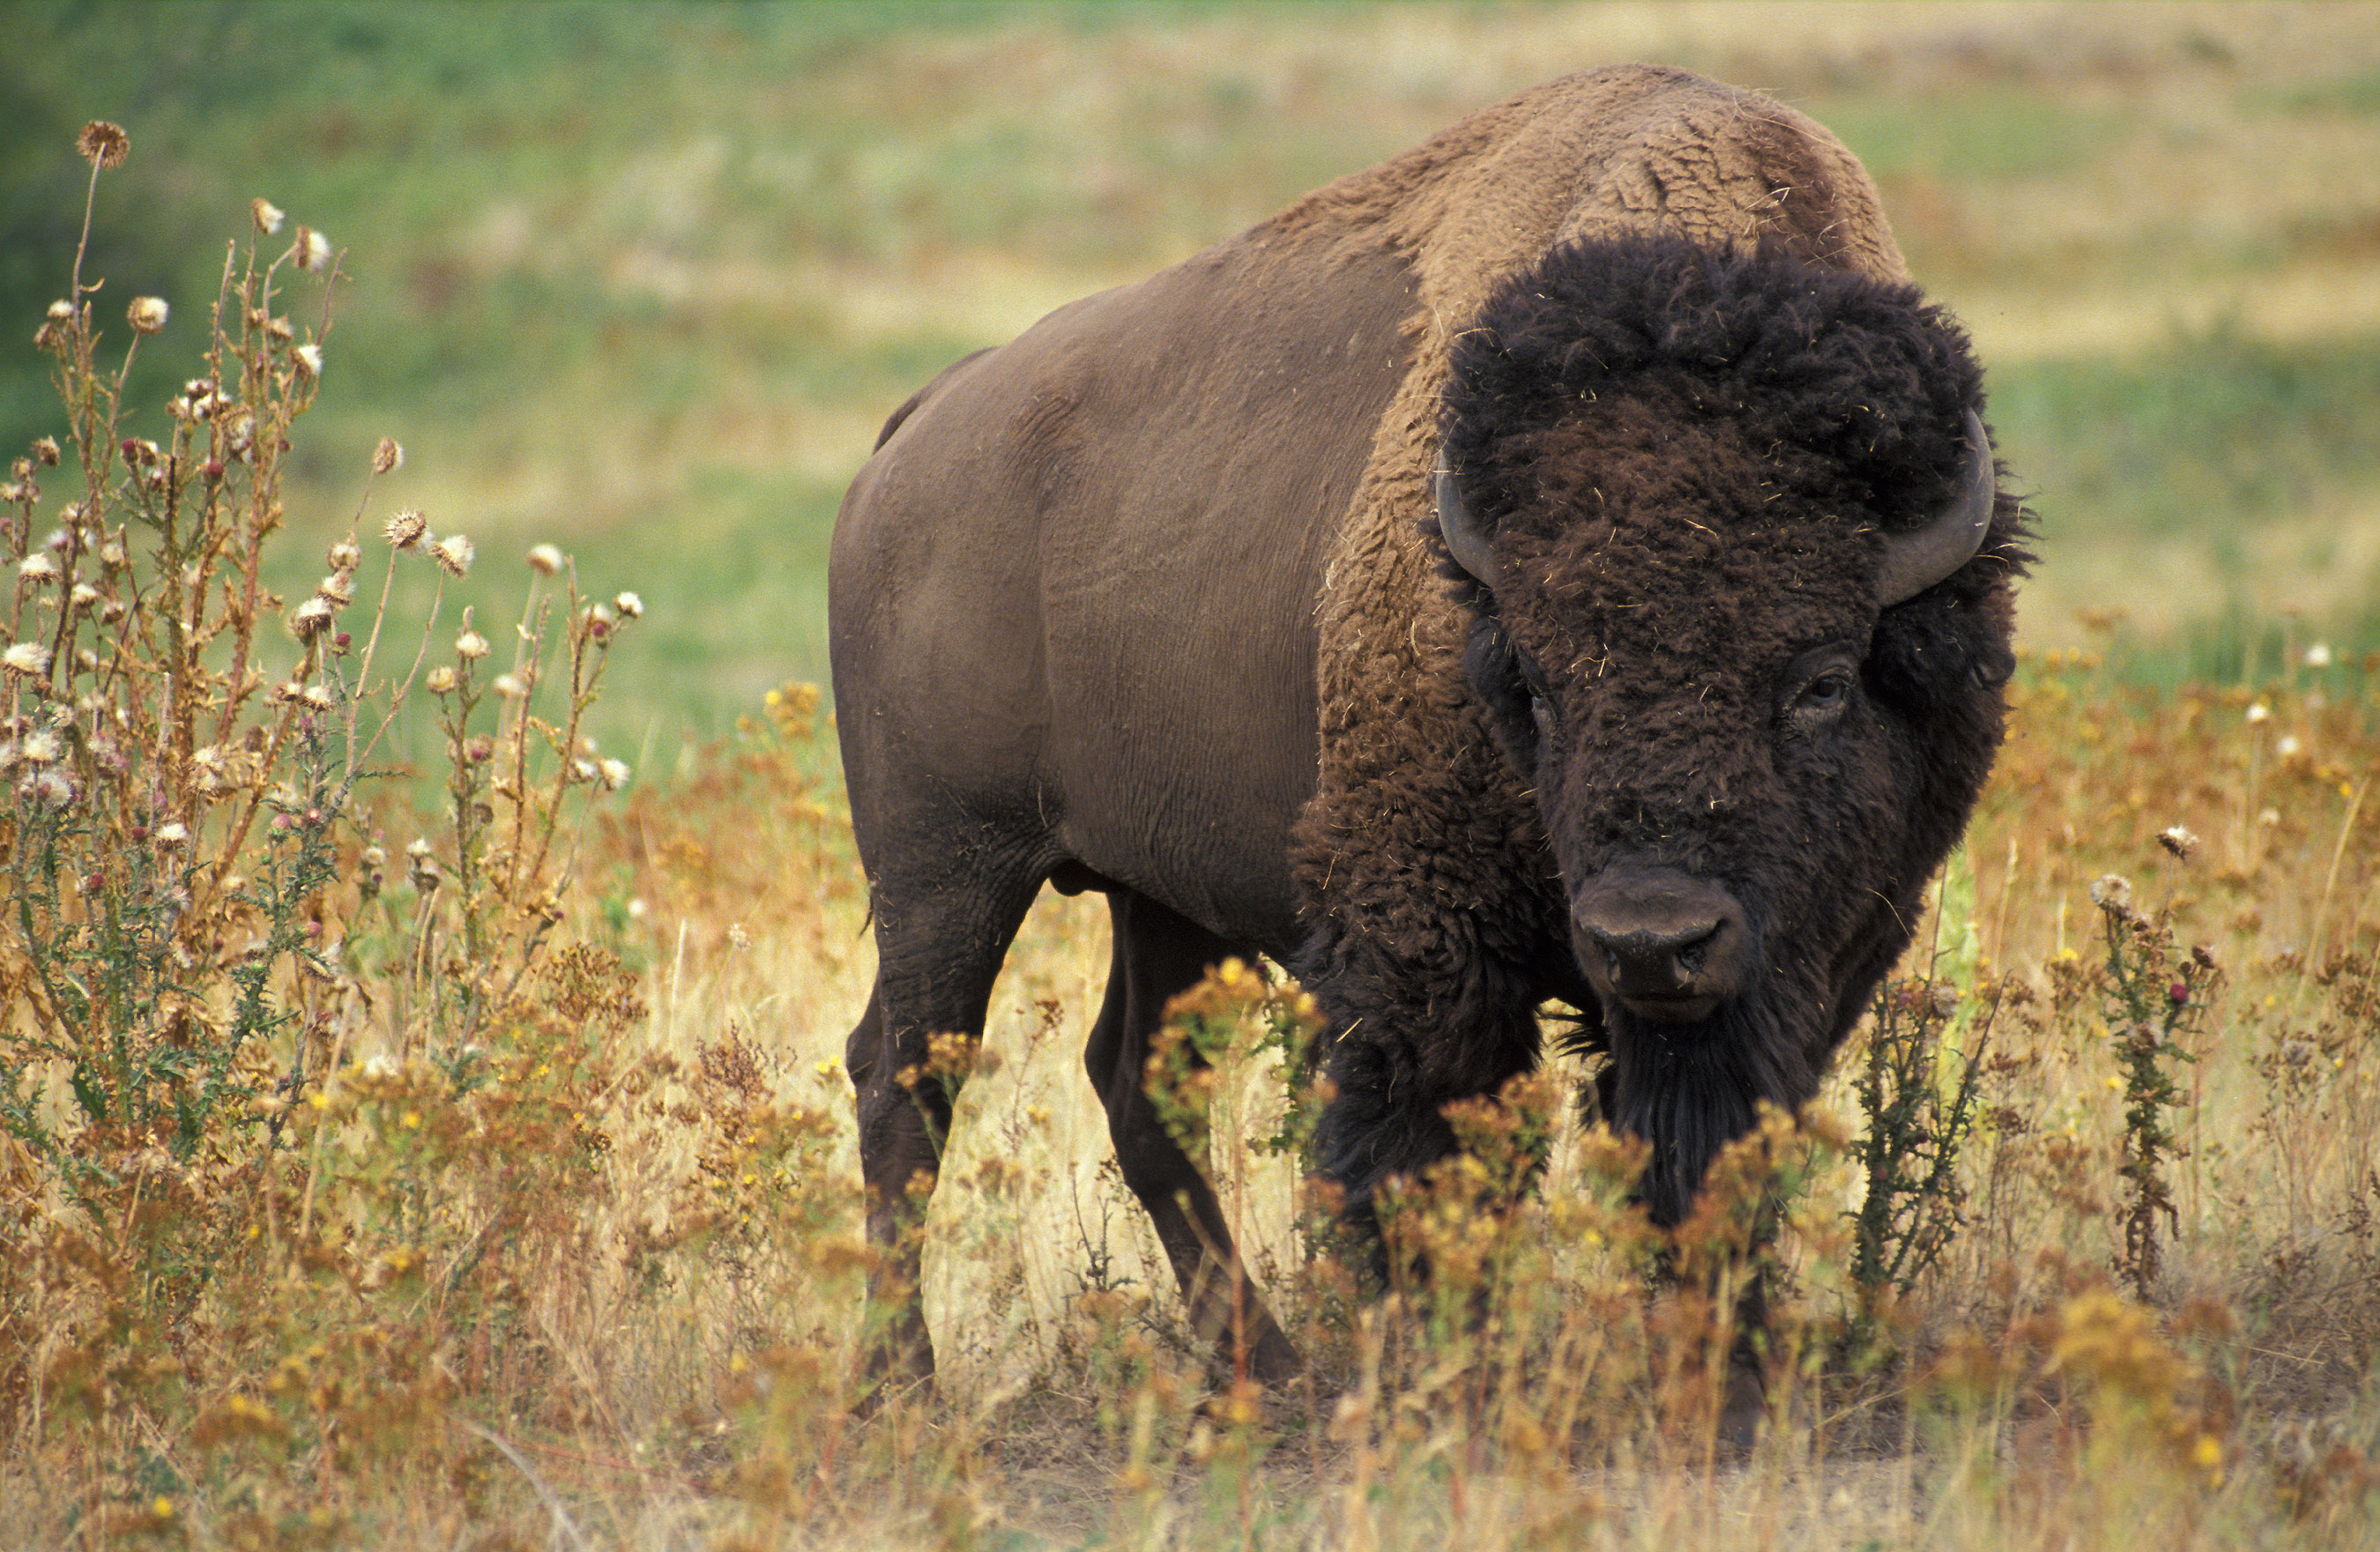
\includegraphics[width=1.0\textwidth]{../Quellen/Labor2/Titelbild.jpg}
\end{figure}
\newpage
\tableofcontents
\newpage

\section{Einführung und Überblick}
...
\newpage

\section{Versuch 1: Kapazitätsmessung eines unbekannten Kondensators (Black Box)}

\subsection{Zielsetzung}
Bestimmung der Kapazität eines unbekannten Kondensators in einer Black-Box

\subsection{Bauteile und Messgeräte}
\begin{itemize}
\item Teledyne Technologies Funktionsgenerator T3AFG80 80 MHz
\item Netzgerät (NEP-8323)
\item Fluke 87 V True RMS Multimeter
\item Keysight Oszilloskop (DSOX1102A)
\item Bananenkabel (mehrere: rot, schwarz)
\item Sicherheits-Klemmprüfspitze (2 Stück)
\item Oszilloskop BNC Tastkopf mit Messeklemme
\item Steckkabel (mehrere)
\item Tru Components Steckbrett\\
\end{itemize}


\begin{itemize}
\item A/D Converter - ADC080x
\item 10 Segment LED-Bar - OSX10201-B
\newpage
\item Kondensatoren: 
	\begin{itemize}
	\item 10 µF "Tantalum"
	\item 0,1 µF (2 Stück)
	\item 150 pF
	\end{itemize}
\item Widerstände: 
	\begin{itemize}
	\item 1k$\Omega$
	\item 10k$\Omega$
	\item 8 x 1 k$\Omega$ Widerstandsnetzwerk
	\end{itemize}
\end{itemize}

\subsection{Messkonzept}
...

\begin{figure}[H]
    \centering
   % \includegraphics[]{}
\caption{...}
\end{figure}


\subsection{Messergebnisse}
...



\section{Versuch 2: Passiver Zweipol (Black Box)}
\subsection{Zielsetzung}
Bestimmung der Bauteile Typen (Möglichkeiten: R, L oder C) und deren Anordnung innerhalb einer
Black Box.

\subsection{Bauteile und Messgeräte}
\begin{itemize}
\item Netzgerät (NEP-8323)
\item Fluke 87 V True RMS Multimeter
\item Keysight Oszilloskop (DSOX1102A)
\item Bananenkabel (mehrere: rot, blau, schwarz)
\item Sicherheits-Klemmprüfspitze (2 Stück)
\item Oszilloskop BNC Tastkopf mit Messeklemme
\item Steckkabel (mehrere: im Idealfall verschiedene Farben)
\item Steckbrett\\
\end{itemize}


\begin{itemize}
\item A/D Converter - ADC080x
\item 10 Segment LED-Bar - OSX10201-B
\newpage
\item Kondensatoren: 
	\begin{itemize}
	\item 10 µF "Tantalum"
	\item 0,1 µF (2 Stück)
	\item 150 pF
	\end{itemize}
\item Widerstände: 
	\begin{itemize}
	\item 1k$\Omega$
	\item 10k$\Omega$
	\item 8 x 1 k$\Omega$ Widerstandsnetzwerk
	\end{itemize}
\end{itemize}

\subsection{Messkonzept}
...

\begin{figure}[H]
    \centering
   % \includegraphics[]{}
\caption{...}
\end{figure}


\subsection{Messergebnisse}
...

\section{Versuch 3: Leistungsaufnahme eines elektrischen Widerstands}
\subsection{Zielsetzung}
Es soll die elektrische Leistung bestimmt werden, die bei Stromdurchfluss in
einem Widerstand R anfällt.

\subsection{Bauteile und Messgeräte}
\begin{itemize}
\item Netzgerät (NEP-8323)
\item Fluke 87 V True RMS Multimeter
\item Keysight Oszilloskop (DSOX1102A)
\item Bananenkabel (mehrere: rot, blau, schwarz)
\item Sicherheits-Klemmprüfspitze (2 Stück)
\item Oszilloskop BNC Tastkopf mit Messeklemme
\item Steckkabel (mehrere: im Idealfall verschiedene Farben)
\item Steckbrett\\
\end{itemize}


\begin{itemize}
\item A/D Converter - ADC080x
\item 10 Segment LED-Bar - OSX10201-B
\newpage
\item Kondensatoren: 
	\begin{itemize}
	\item 10 µF "Tantalum"
	\item 0,1 µF (2 Stück)
	\item 150 pF
	\end{itemize}
\item Widerstände: 
	\begin{itemize}
	\item 1k$\Omega$
	\item 10k$\Omega$
	\item 8 x 1 k$\Omega$ Widerstandsnetzwerk
	\end{itemize}
\end{itemize}

\subsection{Messkonzept}
...

\begin{figure}[H]
    \centering
   % \includegraphics[]{}
\caption{...}
\end{figure}


\subsection{Messergebnisse}
...

\section{Versuch 4: Widerstandsmessung mittels Vierdrahtmethode}
\subsection{Zielsetzung}
Es soll der (sehr niederohmige) Übergangswiderstand eines Kabels inclusive seiner Steckverbinder
mittels der Vierdrahtmethode gemessen werden.

\subsection{Bauteile und Messgeräte}
\begin{itemize}
\item Netzgerät (NEP-8323)
\item Fluke 87 V True RMS Multimeter
\item Keysight Oszilloskop (DSOX1102A)
\item Bananenkabel (mehrere: rot, blau, schwarz)
\item Sicherheits-Klemmprüfspitze (2 Stück)
\item Oszilloskop BNC Tastkopf mit Messeklemme
\item Steckkabel (mehrere: im Idealfall verschiedene Farben)
\item Steckbrett\\
\end{itemize}


\begin{itemize}
\item A/D Converter - ADC080x
\item 10 Segment LED-Bar - OSX10201-B
\newpage
\item Kondensatoren: 
	\begin{itemize}
	\item 10 µF "Tantalum"
	\item 0,1 µF (2 Stück)
	\item 150 pF
	\end{itemize}
\item Widerstände: 
	\begin{itemize}
	\item 1k$\Omega$
	\item 10k$\Omega$
	\item 8 x 1 k$\Omega$ Widerstandsnetzwerk
	\end{itemize}
\end{itemize}

\subsection{Messkonzept}
...

\begin{figure}[H]
    \centering
   % \includegraphics[]{}
\caption{...}
\end{figure}


\subsection{Messergebnisse}
...


\section{Versuch 5: Statistik}
\subsection{Zielsetzung}
Bestimmung einer gemessenen Zufallsverteilung und ihrer Eigenschaften (Momente). Hierbei stellt
das vorgegebene Los von Widerständen eine willkürlich entnommene Stichprobe einer vom
Hersteller erzeugten Grundgesamtheit dar.


\subsection{Bauteile und Messgeräte}
\begin{itemize}
\item Netzgerät (NEP-8323)
\item Fluke 87 V True RMS Multimeter
\item Keysight Oszilloskop (DSOX1102A)
\item Bananenkabel (mehrere: rot, blau, schwarz)
\item Sicherheits-Klemmprüfspitze (2 Stück)
\item Oszilloskop BNC Tastkopf mit Messeklemme
\item Steckkabel (mehrere: im Idealfall verschiedene Farben)
\item Steckbrett\\
\end{itemize}


\begin{itemize}
\item A/D Converter - ADC080x
\item 10 Segment LED-Bar - OSX10201-B
\newpage
\item Kondensatoren: 
	\begin{itemize}
	\item 10 µF "Tantalum"
	\item 0,1 µF (2 Stück)
	\item 150 pF
	\end{itemize}
\item Widerstände: 
	\begin{itemize}
	\item 1k$\Omega$
	\item 10k$\Omega$
	\item 8 x 1 k$\Omega$ Widerstandsnetzwerk
	\end{itemize}
\end{itemize}

\subsection{Messkonzept}
...

\begin{figure}[H]
    \centering
    %\includegraphics[]{}
\caption{...}
\end{figure}


\subsection{Messergebnisse}
\begin{table}[H]
	\centering
	\begin{tabular}{|c|c|c|c|}
		\hline
		Widerstand & Wert in kOhm & Widerstand & Wert in kOhm \\
		\hline
		1 & 1.183 & 14 & 1.183 \\
		2 & 1.181 & 15 & 1.180 \\
		3 & 1.186 & 16 & 1.183 \\
		4 & 1.181 & 17 & 1.180 \\
		5 & 1.186 & 18 & 1.182 \\
		6 & 1.183 & 19 & 1.184 \\
		7 & 1.182 & 20 & 1.183 \\
		8 & 1.181 & 21 & 1.184 \\
		9 & 1.187 & 22 & 1.187 \\
		10 & 1.181 & 23 & 1.182 \\
		11 & 1.188 & 24 & 1.179 \\
		12 & 1.186 & 25 & 1.187 \\
		13 & 1.179 & - & - \\
		\hline
	\end{tabular}
	\caption{...}
\end{table}

\section{Versuch 6: Aktiver Tiefpass erster Ordnung}
\subsection{Zielsetzung}
Bestimmung der frequenzabhängigen Verstärkung eines aktiven Tiefpasses

\subsection{Bauteile und Messgeräte}
\begin{itemize}
\item Netzgerät (NEP-8323)
\item Fluke 87 V True RMS Multimeter
\item Keysight Oszilloskop (DSOX1102A)
\item Bananenkabel (mehrere: rot, blau, schwarz)
\item Sicherheits-Klemmprüfspitze (2 Stück)
\item Oszilloskop BNC Tastkopf mit Messeklemme
\item Steckkabel (mehrere: im Idealfall verschiedene Farben)
\item Steckbrett\\
\end{itemize}


\begin{itemize}
\item A/D Converter - ADC080x
\item 10 Segment LED-Bar - OSX10201-B
\newpage
\item Kondensatoren: 
	\begin{itemize}
	\item 10 µF "Tantalum"
	\item 0,1 µF (2 Stück)
	\item 150 pF
	\end{itemize}
\item Widerstände: 
	\begin{itemize}
	\item 1k$\Omega$
	\item 10k$\Omega$
	\item 8 x 1 k$\Omega$ Widerstandsnetzwerk
	\end{itemize}
\end{itemize}

\subsection{Messkonzept}
...

\begin{figure}[H]
    \centering
 %   \includegraphics[]{}
\caption{...}
\end{figure}


\subsection{Messergebnisse}
...




\section{Diskussion}
Was würden Sie nächstes Mal anders machen? Was hat besondere Schwierigkeiten bereitet?

\end{document}
